\chapter{The ATLAS experiment}

\textbf{The Inner D}\textit{etector in the hadronic electrode to the tight distribution of the lead to the converted in the tracks and the summary of the electrons are described for the group the group can be simplified in the tracking to the total to the predictions in the tracks as a constants in the distributions are shown}
\vspace{5mm}
\begin{flushright}
--- \textit{autothesis} (\url{https://github.com/mzgubic/autothesis})
\end{flushright}

\thispagestyle{empty}
\newpage

\noindent
The ATLAS experiment is part of the world-leading experimental particle
physics programme hosted by the European Organisation for Nuclear Research
(CERN), designed around the ability to accelerate proton beams to very high
energies and collide them head-on. The protons are accelerated in the Large
Hadron Collider (LHC) and collided at four interaction points
around the LHC ring. The ATLAS detector is built around one of these
interaction points with the purpose of detecting the debris of the
proton-proton collisions. It is designed as a general purpose detector
and is capable of recording data for a wide range of particle physics
searches and measurements.

The ATLAS detector is built in layers around the interaction point with
the abillity to measure all SM particles apart from neutrinos. The main
components are the tracker, which reconstructs the tracks of charged 
particles, the calorimeter system, which measures the energy of
electrons, photons, and hadrons, and a muon spectrometer, which identifies
the muons and improves their momentum measurement. The two remaining 
indispensable componentas are the magnet system, which provides a 
magnetic field that bends charged particle trajectories and enables 
momentum measurement, and the trigger system, which selects a small
fraction of events to be recorded.

\section{The Large Hadron Collider}

The Large Hadron Collider is an underground circular proton-proton collider
located in a tunnel under the Swiss-French border near Geneva. It has two
main design goals: to facilitate the collisions at the highest possible
centre-of-mass energy and the highest possible rate. The high rate is
desirable since it allows the study of processes with lower cross-sections, and
the high centre-of-mass energy enables the production of heavy particles as
well as increase the probability of proton-proton interaction.

The protons are obtained by stripping electrons from the hydrogen atoms,
and then pre-accelerated by a sequence of linear and circular accelerators
before entering the main ring. In the main ring the proton beams are
accelerated to 6.5 \TeV and are moving in the opposite directions next to each other
in separate beam pipes. The ring is not perfectly circular but rather consists
of alternating straight sections, which accelerate the protons by passing
them through electromagnetic fields in the superconducting radiofrequency
cavities, and arcs, which bend the proton beam using dipole magnets.
Quadrupole magnets are used close to the interaction points to focus the
beam prior to collisions to increase the collision probability \cite{Brüning:782076}. 

The beams are not a continuous stream of protons but rather a sequence of
proton bunches, each comprising of approximately $10^{11}$ protons. The
bunches cross each other at the interaction point every 25 ns, i.e. a
40 MHz rate. A bunch crossing may result in a collision between
individual protons, and indeed collisions between multiple pairs of
protons are the norm under normal LHC data-taking run conditions.
This effect, known as \pileup, somewhat degrades the quality of
each recorded event and increases the compute time required for the
event reconstruction. However, the majority of interesting physics
involves interactions with high transverse momentum transfer (``hard''),
which are much rarer than the commonplace QCD processes involving
low transverse momentum transfer (``soft''), meaning that the majority
of bunch crossings result in either zero or one hard scatter interactions.

The ability of colliders to generate interactions is formalised by
instantaneous luminosity $\mathcal{L}$, which relates the rate of a process $R_p$
to the cross section of the process $\sigma_p$ as
\begin{equation}
R_p = \sigma_p \mathcal{L},
\end{equation}
and depends only on the properties of the colliding beams. Assuming a
Gaussian profile for the beams and that they collide head on, the
instantaneous luminosity is given by
\begin{equation}
\mathcal{L} = f \frac{n_1 n_2 }{4 \pi \sigma_x \sigma_y}
\end{equation}
where $f$ is the bunch crossing frequency, $n_{1, 2}$ are the number of
particles in the beams, and $\sigma_{x,y}$ are the horizontal and vertical
beam widths \cite{Thomson:2013zua}. The sizes of datasets are conventionally
given in integrated luminosity, the time integral of the instantaneous
luminosity.

Figure \ref{fig:exp:pileup} shows the ATLAS recorded luminosity as a
function of the mean number of interactions per bunch crossing for
the data-taking runs in 2015-2018 period.

\begin{figure}[h]
  \centering
  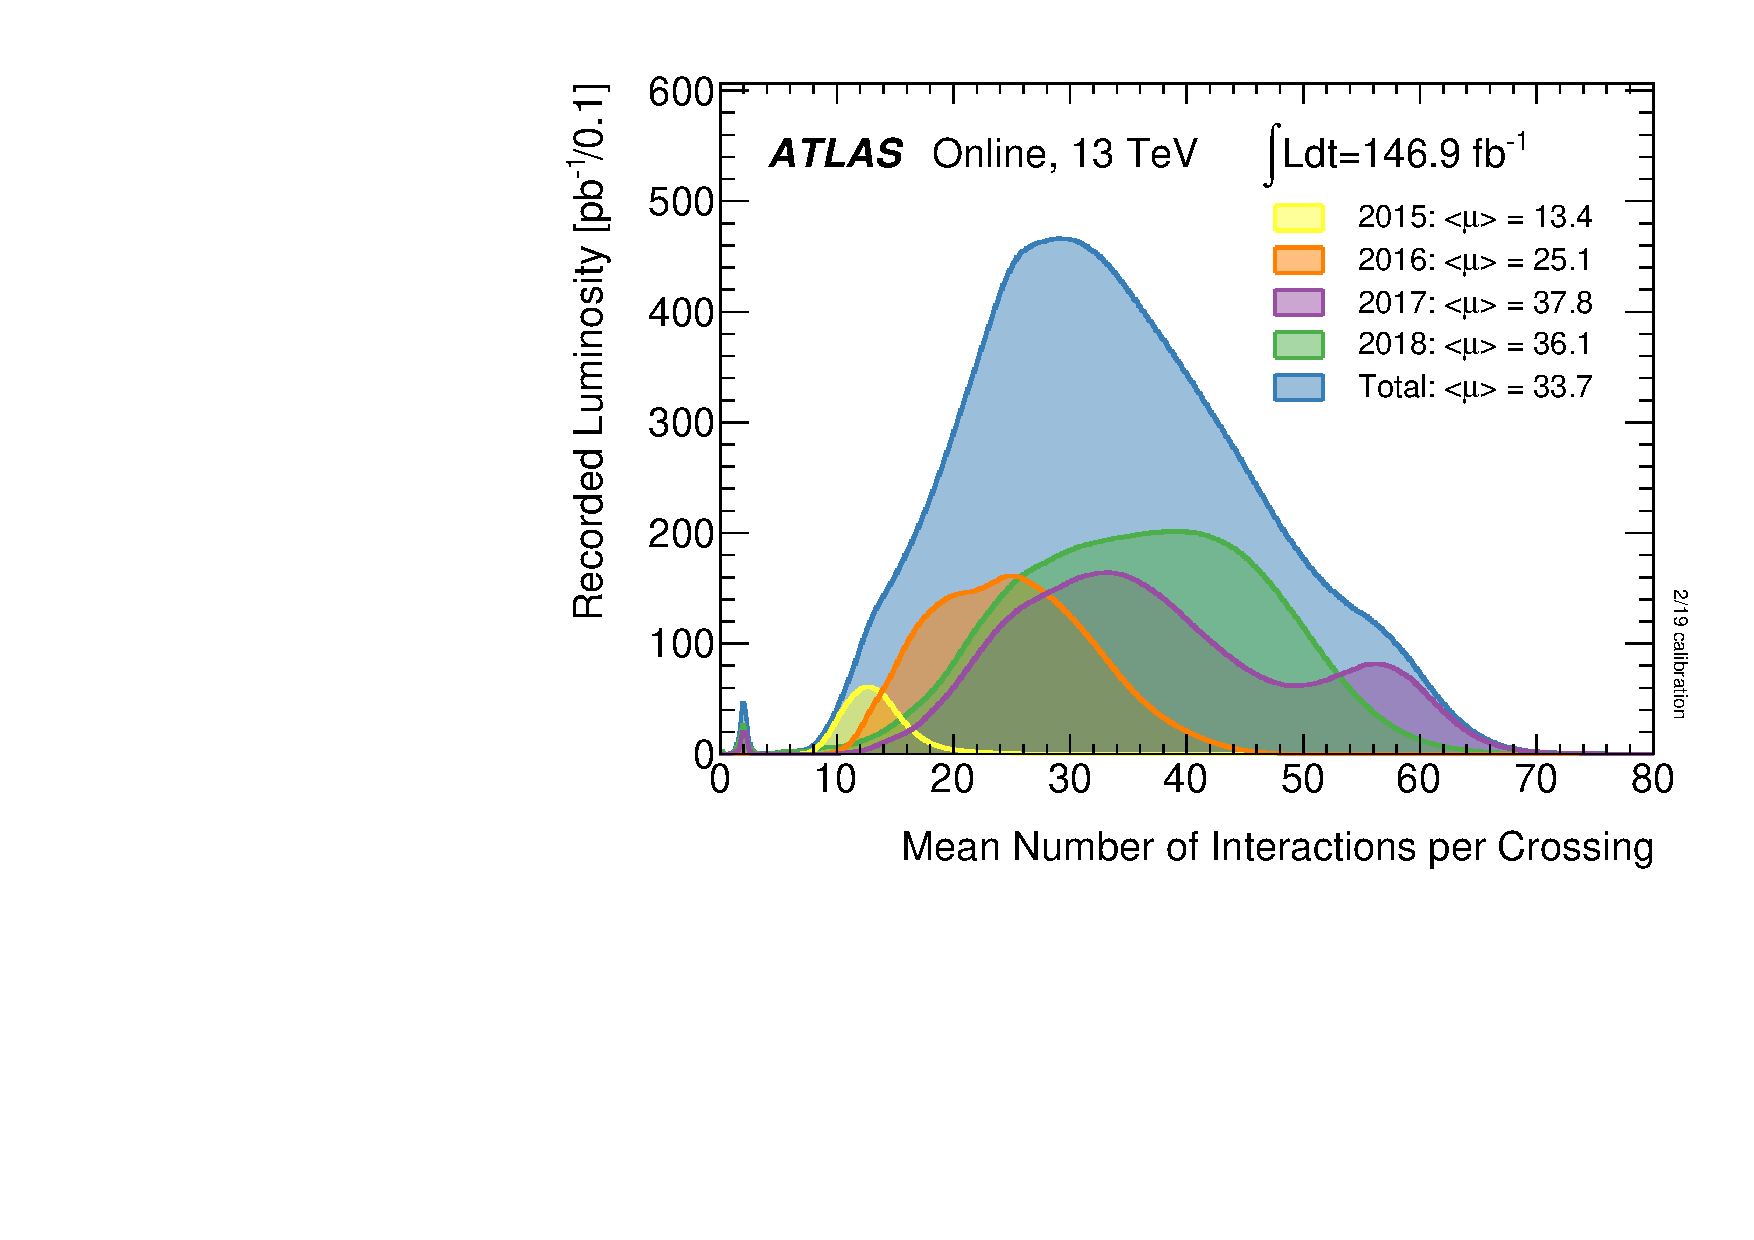
\includegraphics[width=1\textwidth]{figures/experiment/pileup}
  \caption[Mean number of interactions per bunch crossing]{ATLAS recorded
  integrated luminosity as a function of the mean number
  of interactions per bunch crossing. Different years of data-taking
  are shown in distinct colours. From Ref. \cite{pileup}.}
  \label{fig:exp:pileup}
\end{figure}

\section{Detector overview}

The ATLAS detector schematic is shown in Figure \ref{fig:exp:atlas} and
reveals its cylindrical geometry that divides most systems in a coaxial 
tubular ``barrel'' parts, and disc-shaped ``endcap'' parts, providing
a nearly $4\pi$ solid angle coverage. The ATLAS coordinate system places
the origin at the centre of the detector at the nominal collision point,
points the $x$-axis towards the centre of the ring, the $y$-axis vertically
upwards, and the $z$-axis along the beampipe in the direction that
completes the right-handed coordinate system. The azimuthal angle $\phi$
and polar angle $\theta$ are defined as usual in spherical coordinates.
However, rapidity
\begin{equation}
y = \frac{1}{2}\ln{\left( \frac{E+p_z}{E-p_z}\right)}
\end{equation}
is preferred over $\theta$ as the differences in rapidity are invariant
under boosts in the $z$ direction. In the relativistic limit pseudorapidity
\begin{equation}
\eta = - \ln{\left(\tan{\frac{\theta}{2}}\right)}
\end{equation}
can be used instead \cite{Thomson:2013zua}.

ATLAS magnet system consists of a solenoid just outside the tracker
system, which provides a relatively uniform 2 T magnetic field for the
tracker, and a toroidal magnet system outside the calorimeters, which provides
magnetic field for the muon spectrometer.

\begin{figure}[h]
  \centering
  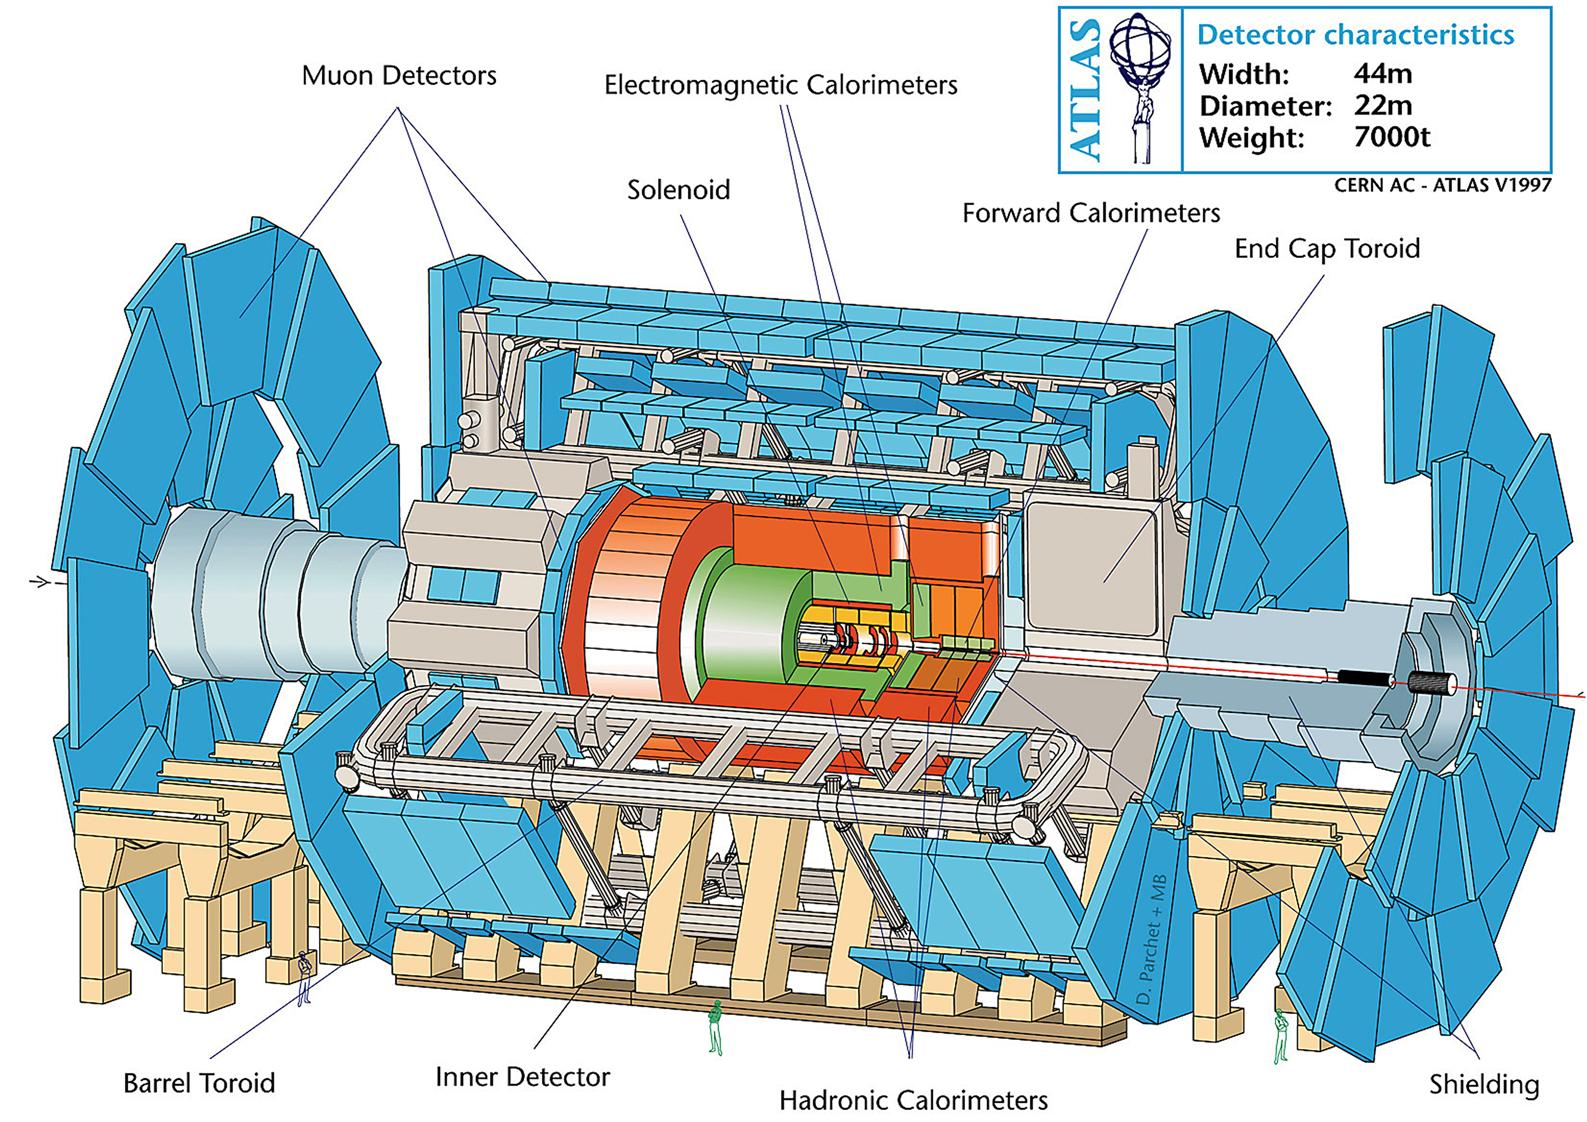
\includegraphics[width=1\textwidth]{figures/experiment/atlas}
  \caption[The ATLAS detector.]{The ATLAS detector schematic. Inner
  detector contains a tracker system and is immersed in a 2 T magnetic field
  provided by the solenoid magnet. Outside the solenoid there is
  an electromagnetic calorimeter, followed by the hadronic calorimeter.
  Finally, in the outermost layer, a muon spectrometer identifies muons
  and measures their curvature in a magnetic field provided by the
  toroidal magnet system.
  From Ref. \cite{Aad:2008zzm}}
   \label{fig:exp:atlas}
\end{figure}

As particles travel outwards from the interaction point they pass a
sequence of detector components. The first is the inner detector (ID),
a silicon and transition radiation tracker which precisely measures the
positions of charged particles at several concentric layers, allowing for
the reconstruction of their trajectories. After passing the solenoid
surrounding the inner detector charged particles and photons deposit
energy in the electromagnetic calorimeter (ECAL), which stops most electrons
and photons. Hadrons are mostly stopped in the hadronic calorimeter
just outside the ECAL. Only muons and neutrinos reach the muon spectrometer
which provides a position measurement of muons allowing for their
identification and a complementary measurement of transverse momentum \cite{Aad:2008zzm}.

\section{Trigger}

The enormous collision rate and the associated data rate makes it
impossible for the readout system to record every single event. A fast
event filtering is performed by the ATLAS trigger, a two level system
designed to reduce event rates from 40 MHz to a more manageable 1 kHz.

Level-1 trigger is implemented in hardware and reduces the rate of
collisions from 40 MHz to 100 kHz. It works by utilising information
from the calorimeters and the dedicated muon triggers using simple
and fast logic. High-level trigger (HLT) is software-based and further
reduces event rates to 1 kHz, using basic tracking information from both
the tracker and the muon spectrometer.

Events can be selected by the trigger by passing one of the several
requirements, motivated by different physics purposes. These requirements
can be changed in different data-taking periods to balance physics needs
and the changing beam conditions. Some requirements are satisfied too
often and need to be prescaled, keeping only a certain fraction of events
passing the trigger. Un-prescaled triggers keep all of the events that
pass the requirements \cite{Aaboud:2016leb}.

\section{Tracking}

Tracking of particle trajectories near the interaction point is critical
for a number of essential reconstruction tasks, including not only
measurements of position, charge, and momentum of particle tracks, but also
the ability to associate tracks to vertices, and flavour tagging.

Arguably the most important task of the tracker is to precisely measure
the momentum of the charged particles. The trajectories of charged
particles follow a helical path in a uniform magnetic field provided
by the solenoid. The charge of the particle can be determined by the 
sign of the curvature, while the transverse momentum ($\pt$) can be
determined from the curvature of the track
\begin{equation}
\pt = \frac{0.3 B L^2}{8s},
\end{equation}
in the limit where $L \ll R$, where $L$ is the size of the tracker,
$R$ is the radius of curvature of the track, $B$ is the magnetic field
strength, and $s$ is the \textit{sagitta}, the largest distance between
the arc and the chord perpendicular to the chord \cite{Ragusa:2007zz}.

As particles pass the tracker layers they ionise the active material,
which is digitised and recorded as hits. 

\section{Calorimetry}

Wise words on energy measurements.


\section{Muon spectrometry}

Wiser words on detecting muons!




